%%%%%%%%%%%%%%%%%%%%%%%%%%%%%%%%%%%%%%%%%
% Developer CV
% LaTeX Template
% Version 1.0 (28/1/19)
%
% This template originates from:
% http://www.LaTeXTemplates.com
%
% Authors:
% Jan Vorisek (jan@vorisek.me)
% Based on a template by Jan Küster (info@jankuester.com)
% Modified for LaTeX Templates by Vel (vel@LaTeXTemplates.com)
%
% License:
% The MIT License (see included LICENSE file)
%
%%%%%%%%%%%%%%%%%%%%%%%%%%%%%%%%%%%%%%%%%

%----------------------------------------------------------------------------------------
%	PACKAGES AND OTHER DOCUMENT CONFIGURATIONS
%----------------------------------------------------------------------------------------

\documentclass[9pt]{developercv} % Default font size, values from 8-12pt are recommended

%----------------------------------------------------------------------------------------

\begin{document}

%----------------------------------------------------------------------------------------
%	TITLE AND CONTACT INFORMATION
%----------------------------------------------------------------------------------------

\begin{minipage}[t]{0.45\textwidth} % 45% of the page width for name
	\vspace{-\baselineskip} % Required for vertically aligning minipages

	% If your name is very short, use just one of the lines below If your
	% name is very long, reduce the font size or make the minipage wider
	% and reduce the others proportionately
	\colorbox{black}{{\HUGE\textcolor{white}{\textbf{\MakeUppercase{Samuel}}}}} % First name

	\colorbox{black}{{\HUGE\textcolor{white}{\textbf{\MakeUppercase{Kyletoft}}}}} % Last name

	\vspace{6pt}

	% {\huge Computer} % Career or current job title
\end{minipage}
\begin{minipage}[t]{0.275\textwidth} % 27.5% of the page width for the first row of icons
	\vspace{-\baselineskip} % Required for vertically aligning minipages
	
	% The first parameter is the FontAwesome icon name, the second is the
	% box size and the third is the text Other icons can be found by
	% referring to fontawesome.pdf (supplied with the template) and using
	% the word after \fa in the command for the icon you want
	\icon{MapMarker}{12}{Göteborg}\\
	\icon{Phone}{12}{+46 761 76 53 67}\\
	\icon{At}{12}{\href{mailto:samuel@kyletoft.se}{samuel@kyletoft.se}}\\	
\end{minipage}
\begin{minipage}[t]{0.275\textwidth} % 27.5% of the page width for the second row of icons
	\vspace{-\baselineskip} % Required for vertically aligning minipages
	
	% The first parameter is the FontAwesome icon name, the second is the
	% box size and the third is the text Other icons can be found by
	% referring to fontawesome.pdf (supplied with the template) and using
	% the word after \fa in the command for the icon you want
	\icon{Globe}{12}{\href{https://samuel.kyletoft.se}{samuel.kyletoft.se}}\\
	\icon{Github}{12}{\href{https://github.com/SKyletoft}{/SKyletoft}}\\
	\icon{Linkedin}{12}{\href{https://www.linkedin.com/in/samuel-kyletoft}{/samuel-kyletoft}}\\
\end{minipage}

\vspace{0.5cm}

%----------------------------------------------------------------------------------------
%	INTRODUCTION, SKILLS AND TECHNOLOGIES
%----------------------------------------------------------------------------------------


\begin{minipage}[t]{0.8\textwidth} % 40% of the page width for the introduction text
	\vspace{-\baselineskip} % Required for vertically aligning minipages
	\cvsect{Vem är jag?}

	Född 2000 i Stockholm och nuvarande student på Chalmers Tekniska
	Högskola. \\Fokuserad på kompilatorer och prestanda.
\end{minipage}
\hfill % Whitespace between
\begin{minipage}[t]{0.2\textwidth} % 50% of the page for the skills bar chart
	\vspace{-\baselineskip} % Required for vertically aligning minipages
	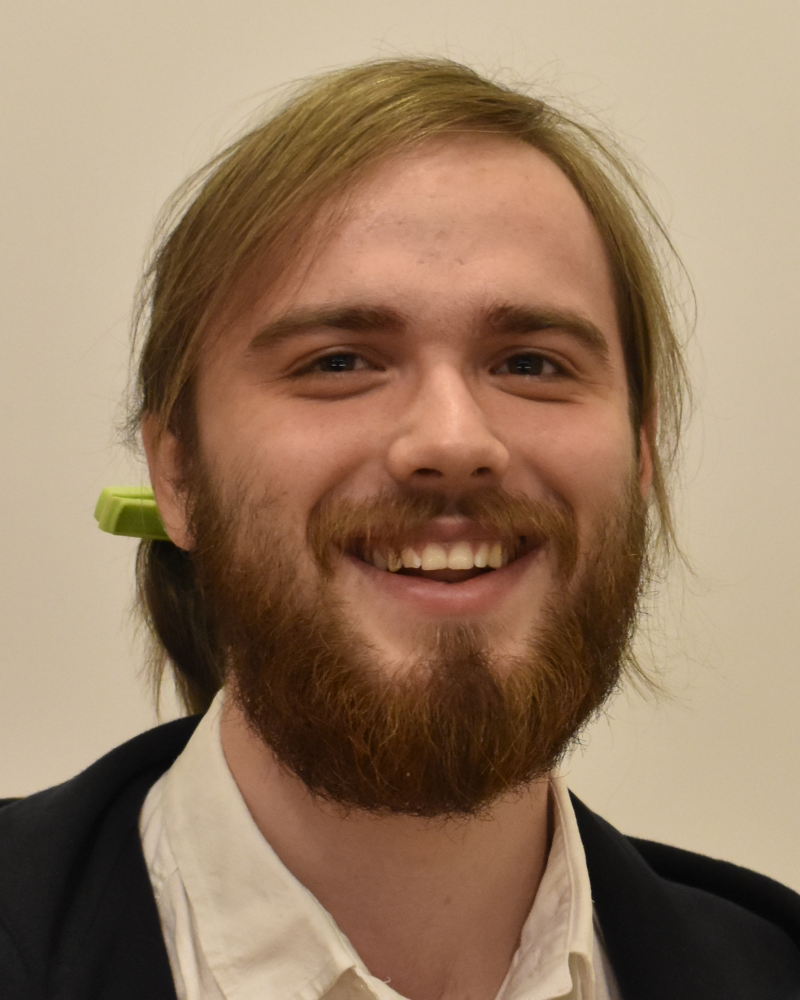
\includegraphics[width=\linewidth]{smaller.png}
\end{minipage}

%----------------------------------------------------------------------------------------
%	EXPERIENCE
%----------------------------------------------------------------------------------------

\cvsect{Erfarenhet}

\begin{entrylist}
	\entry
		{8/2021 -- }
		{Lärarassistent (TA)}
		{Chalmers Tekniska Högskola}
		{
			Som lärarassistent har jag drivit labbpass, hjälpt studenter i
			kurserna och rättat tentor och labbar.\\
			\texttt{Introduktion till funktionell programmering}\slashsep
			\texttt{Grundläggande datorteknik}\slashsep
			\texttt{Maskinorienterad programmering}\slashsep
			\texttt{Introduktion till Objektorienterad programmering}\slashsep
			\texttt{Principer för Parallell programmering}
		}
	\entry
		{5/2022 -- }
		{Ledamot}
		{Datateknologsektionens Arbetsmarknadsgrupp, DAG}
		{Som ledamot i DAG har jag varit en av Datateknologsektionens
		kontaktpersoner utåt mot arbetslivet. Vi har arrangerat
		lunchföreläsningar, pubkvällar och resor för att besöka
		företag.\\}
	\entry
		{5/2021 -- 5/2022}
		{Mikrodatordriftsystemsergeant}
		{Datateknologsektionens serverkommitée, dHack}
		{I mitt år i dHack har jag driftat Datateknologsektionens
		servrar och tjänster, samt startat nya.\\}
\end{entrylist}

%----------------------------------------------------------------------------------------
%	EDUCATION
%----------------------------------------------------------------------------------------

\cvsect{Utbildning}

\begin{entrylist}
	\entry
		{2020 -- }
		{(Pågående) Civilingenjör Datateknik, 300hp}
		{Chalmers Tekniska Högskola}
		{}
	\entry
		{2020 VT}
		{Juridisk Översiktskurs, 15hp}
		{Uppsala Universitet}
		{}
\end{entrylist}

%----------------------------------------------------------------------------------------
%	ADDITIONAL INFORMATION
%----------------------------------------------------------------------------------------

\begin{minipage}[t]{0.3\textwidth}
	\vspace{-\baselineskip} % Required for vertically aligning minipages

	\cvsect{Språk}

	\textbf{Svenska} - flytande\\
	\textbf{Engelska} - flytande
\end{minipage}
\hfill
\begin{minipage}[t]{0.6\textwidth}
	\vspace{-\baselineskip} % Required for vertically aligning minipages
	
	\cvsect{Hobbys}
	
	På helger tar jag ofta alldeles för långa skogsprommenader och jobbar
	på att implementera programspråket Artemis.
\end{minipage}

%----------------------------------------------------------------------------------------

\end{document}
